\documentclass[]{article}

\usepackage{amsmath}
\usepackage{amssymb}
\DeclareMathOperator*{\argmax}{arg\,max}
\DeclareMathOperator*{\argmin}{arg\,min}

\usepackage{setspace}
\linespread{1.5}
\usepackage[margin=1in]{geometry}

\usepackage{graphicx}

%opening
%\title{A Machine Learning Framework for Simultaneous Domain Adaption, Map Estimation, and Representation Learning for Datasets with Domain Variability}
\title{Elastic Feature Learning for Data with Domain Variability}
\author{Michael Wilson}
\date{November 2022}

\begin{document}

\maketitle

\begin{abstract}
We present a general machine learning framework for alignment, feature learning, and classification of data with domain variability. We present results on real and simulated data.  
\end{abstract}

\section{Introduction}

Feature learning, or representation learning, is a set of techniques that allow a system to automatically discover features that enable optimal classification. However, when there exists domain variability in the data points (functions, DTMRI fiber tracts, etc) one wishes to classify, features learned on the domain of one data point don't readily transfer to other data points. In this paper, we propose a general framework for combined feature matching and feature learning for the classification of data with domain variability, using tools from statistical shape analysis and machine learning. 

Key to this work is the fact that in the Elastic Shape Analysis framework, a shape is uniquely defined by the values of its local extrema. As our examples will illustrate, Elastic feature learning after alignment can give simple, interpretable models with high test set accuracy for data whose shapes are drawn from uni-modal shape distributions, but don't work well for multi-modal shape distributions, where different shape distributions may have different features that need to be learned. Conversely, shape distances are useful for separating multi-modal shape distributions into uni-modal clusters, but don't provide as good classification accuracy if only some features of the shape are informative. By using shape distances to separate data into uni-modal clusters, and then applying alignment and feature learning to each cluster individually, we are able to get simple, interpretable models with good classification accuracy on data whose shapes are drawn from multi-modal shape distributions. 

We use 4 examples to illustrate our approach. We start by applying Elastic Feature learning to two uni-modal distributions. The first is the Berkeley Growth Study data, learning Elastic Features in order to classify male and female. The second is a simulated data set, designed to show exactly why Elastic Feature Learning outperforms Elastic distance for classification. We then use two examples of multi-modal distributions; a modified version of the Berkeley Growth study data, intended to show the benefit of clustering shapes, and then an application to classifying PTSD based on DTMRI data.



\section{Uni-modal Shape Distributions}

\subsection{Berkeley Growth Study}

\begin{figure}
	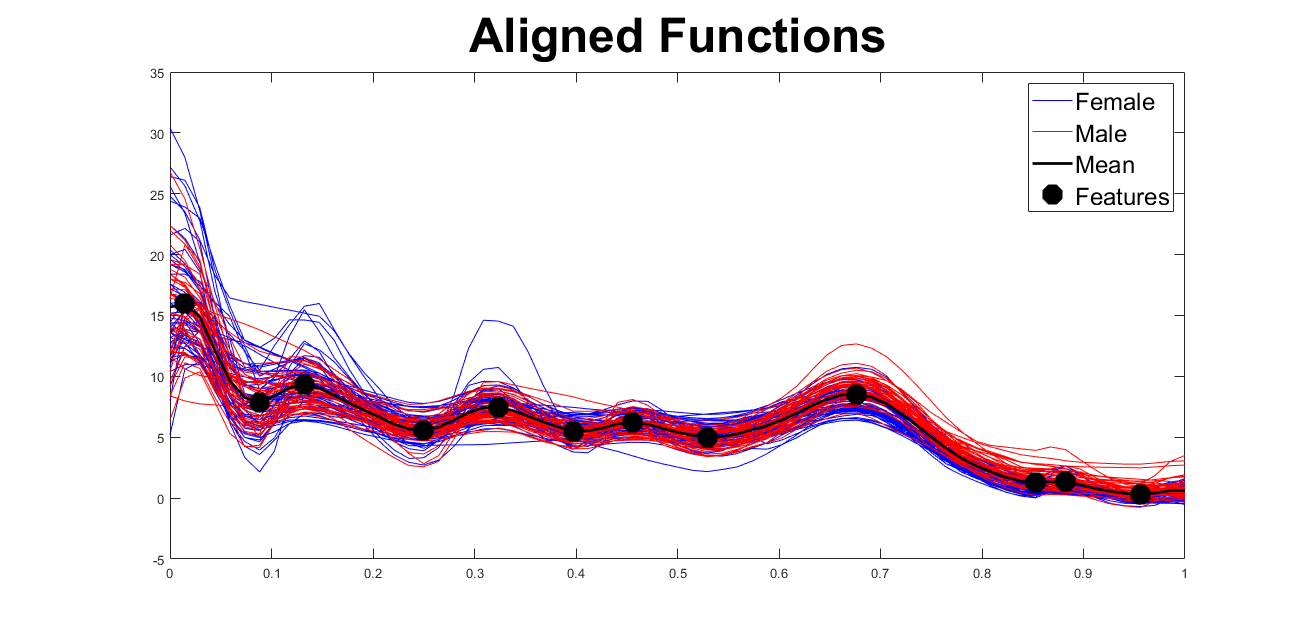
\includegraphics[width = \linewidth]{./Aligned Functions.png}
	\caption{This is the caption}
	\label{aligned function}
\end{figure}

\begin{table}
	\begin{tabular}{|c|c|c|c|c|c|c|c|c|c|c|c|c|c|c|}
		\hline
		\text{Feature:}& 1 & 2 & 3 & 4 & 5 & 6 & 7 & 8 & 9 & 10 & 11 & 12\\
		\hline
		\text{1-cut Tree }&  &  &  &  &  &  &  &  &  &  &  & \\ 
		\text{LOO Accuracy:}& 0.52 & 0.58 & 0.58 & 0.52 & 0.48 & 0.55 & 0.57 & 0.58 & 0.78 & 0.70 & 0.62 & 0.72\\ 
		\hline
	\end{tabular}
	\caption{Even though our feature extraction picks out 12 features, only features 9, 10, and 12 individually achieve higher than 0.7 percent test set accuracy. These scores are used to order our features for forward model selection. Note that 57\% of the labels are female, so 57\% accuracy is no better than chance.}
	\label{feature_LOO}
\end{table}

\begin{figure}
	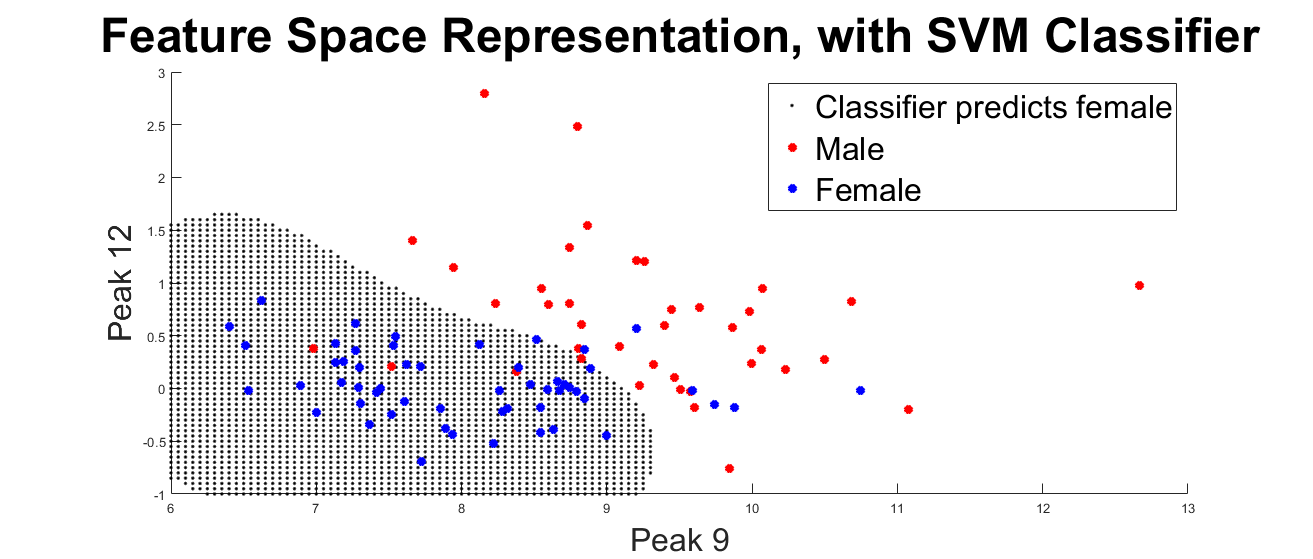
\includegraphics[width = \linewidth]{./Feature Space.png}
	\caption{This is the caption}
	\label{EX1: classifier plot}
\end{figure}


For our first example, we consider classifying the Berkeley Growth Study dataset into male and female. This is not intended to be the optimal application of our approach for this data set; on the contrary, it is intended to be a simple illustration of a much more general pipeline that can be applied to any data set with domain variability. With that in mind, our pipeline for this data set will be as follows;\\

\noindent
1) Domain Adaption: Multiple Alignment\\
2) Elastic Feature Extraction: Select extrema of mean function as features\\
3) Feature Selection: Forward selection, based on 1-cut Decision Tree test set accuracy\\
4) Classification: SVM with Gaussian Kernel for Classification\\

Our first step is to perform multiple alignment on our functions, and calculate a shape mean for the data. Given our shape mean, there are many ways to perform feature extraction. For simplicity, we will just treat the values of our aligned functions at time points corresponding to the local extrema of our shape mean as our features. The results of these steps are presented in Figure $\ref{aligned function}$. 

After alignment, our feature extraction method finds 12 features, denoted with black dots in Figure $\ref{aligned function}$. Now we wish to determine which of our features are informative for classification. There are many ways to measure the informativeness of a feature, with classification accuracy of a 1-cut decision tree being among the simplest. The results of these models are presented in Table \ref{feature_LOO}. Thus, our next step is to use forward selection (forward w.r.t. Leave-One-Out classification accuracy of 1-cut decision trees) to select a subset of maximally informative features, defined in terms of 10-fold cross validation performance.

Figure \ref{EX1: classifier plot} shows the results of running a Gaussian Kernel SVM using only features 9 and 12, the two most common features selected in our validation models (in fact, selected by our learner in every validation model). Our learner achieves just over 86\% Leave-One-Out test set accuracy. Furthermore, the features are very interpretable; feature 9 might be called an 'early puberty high', while feature 12 might be called a 'late puberty low'. Males tend to have higher growth rates at both of these time points, and a classifier built on these two features gets high classification accuracy.

A pipeline using the same model selection criterion, using elastic pairwise distances as features yields a Leave-One-Out classification accuracy of 74.19\%. While this classifier still does better than chance, it has significantly lower classification accuracy, and the features aren't as interpretable. We can show which growth curves are used in the classifier, but are left to speculate what features of a particular growth curve are informative. Note, these results are for a linear SVM; a Gaussian Kernel SVM on our shape distances performs much worse. 

This example shows that Elastic Feature Learning can significantly outperform classification based only on shape distances. Our next example is intended to show exactly why and how Elastic Feature Learning can outperform Elastic distances for classification.  


\subsection{Simulated Uni-modal Shape Distributions}

\begin{figure}
	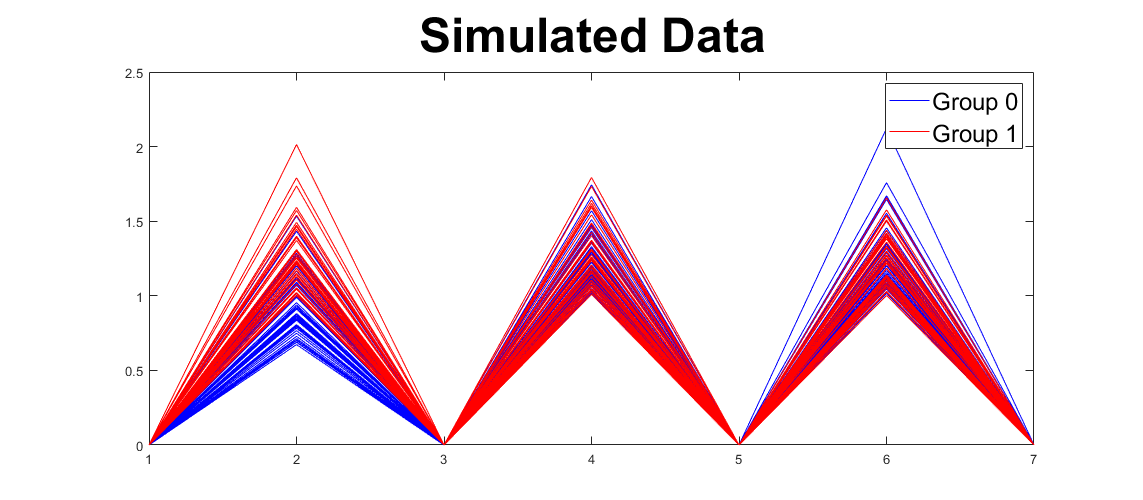
\includegraphics[width = \linewidth]{./simulated data2.png}
	\caption{Even though there is a strong signal in the first peak, it gets drowned out by the second and third peaks when using shape distances as features. Feature Learning attempts to correct for this. }
	\label{simulated data}
\end{figure}

For this example, we will simulate uni-modal functional data, and show that, as the number of uninformative elastic features increases, the classification accuracy of models built on Elastic distances decreases, while Elastic Feature Learning maintains high classification accuracy.  

For simplicity, we will simulate our data as piecewise linear functions, with each time point either a local max or local min. We simulate our data such that only the first peak is informative about class, with the experiment being to see how Elastic Feature Learning compares to classification based on Elastic pairwise distances as we add more uninformative peaks (and thus decrease the signal to noise ratio). Figure \ref{simulated data} shows an example of our simulated data, for M = 3. Specifically, for a function $f_i(t)$, $i = 1,...,n$,  defined over $T=[1,((2*M)+1)]$, labels $\ell_i$, and $\epsilon_i(t) \sim N(0,0.33)$, we simulate;

 \[f_i(t) = \begin{cases} 
	0 & if \text{ t odd} \\
	1 + (0.4)*\ell_i(t) + \epsilon_i(t) & if \text{ t =2}\\
	1 + \epsilon_i(t) & if \text{ t$>2$, t even}
\end{cases}
\]


%We will simulate our data as (unnormalized) sums of $N$ truncated Gaussian pdfs over $[0,1]$ with $M, j = 1,...,M$ mixture components, means $\mu_j = \frac{j}{M+1}$, weights $w_j$, $\sigma^2 = 0.1/M$. For simplicity, mixture component 1 will be the only feature that contains information about our labels $\ell_i$, $i = 1,...,N$, such that for some $\delta \in \mathbb{R}$ and $\epsilon \sim N(0,0.33)$, $w_1(\ell_i) = \frac{1 + \delta\ell_i + \epsilon_i}{M + 1}$, and for $j>1$, $w_j(\ell_i) = \frac{1 + \epsilon_i}{M+1}$. Figure \ref{simulated data} shows an example of data simulated in this way, with M = 3.

The Elastic Distance involves an integral over the entire domain. If there is information about class contained at every point in the domain, the Elastic Distance will be very useful for quantifying that. If, however, only a subset of the domain contains information about the class, as is the case with our simulated data and the single informative peak, then the proportion of the Elastic distance that can be attributed to that informative element will be equal to the proportion of the domain that informative feature(s) are defined over. 
%Specifically, for a function f defined over domain $\mathcal{D}$, with informative features defined only over $\mathcal{I} \subset \mathcal{D}$, we can define a signal-to-noise ratio as;\\
%\begin{equation}
%	S = \frac{\int_\mathcal{I} 1 dt}{\int_\mathcal{D} 1 dt}
%\end{equation}

  Using Elastic Feature Learning, we can learn which portions of the domain to focus on, and thus increase the signal to noise ratio of our features. Figure \ref{simulated data compare} shows the 10-fold CV accuracy of models built using only pairwise Elastic Distances as features, vs Elastic Feature Learning. This analysis is a bit contrived; we restricted our models to 1-cut decision trees, and designed the data so that a 1 cut decision tree based on our approach would converge to the Bayes Optimal predictor as sample size increased. But the feature learning approach consistently selects the informative peak, and thus loses no classification performance as the proportion of uninformative features increases. Classifying based on elastic distances consistently degrades in performance as more uninformative features are added to the data.


	\begin{figure}
		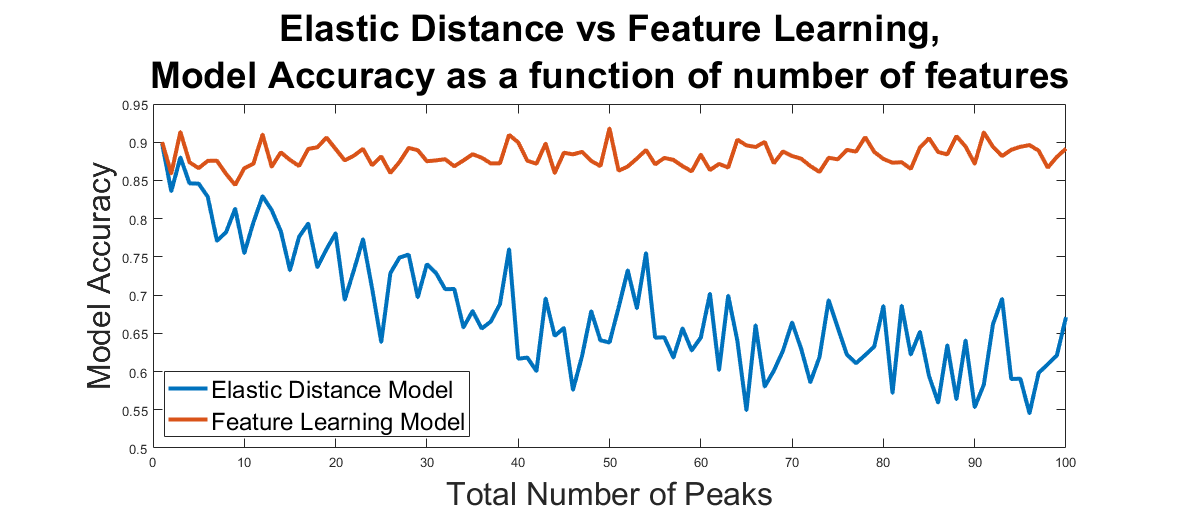
\includegraphics[width = \linewidth]{./simulated_model_compare.png}
		\caption{This is the caption}
		\label{simulated data compare}
	\end{figure}



\section{Multi-modal Shape Distributions}

\subsection{Berkeley Growth Study, with second cluster}

For our second example, we add a second cluster to the Berkeley Growth data, with a distinct shape mean. For simplicity, we take the negative of the original set of growth curves, and then switch the labels, such that if f(t) is a function in the original data set with label 'male', then -f(t) will be added to the dataset, with label 'female'. Figure \ref{aligned function2} shows these curves after alignment. 

Clearly, the shape mean of this data set is less representative of the data than our previous shape mean. Thus, we should expect that features learned from this alignment will be less informative about class than the features learned in our previous alignment. Using the same model as we did in our previous example yields a LOO test set accuracy of just 67.74\%. While this is surprisingly good, it is significantly worse than the 86\% we got in our previous example. Furthermore, because our second cluster is just the negative of our first cluster, we should expect that the classification on each cluster individually would also be 86\%. Thus, if we add a step to our algorithm to first determine clusters based on shape, and then apply our alignment and feature learning to each cluster, we should be able to significantly improve our classification performance. Figure \ref{aligned function2} shows the Elastic pairwise distance matrix, with the first 93 rows corresponding to cluster 1, and the second 93 columns corresponding to cluster 2. Given the method by which we produced the second cluster, it shouldn't be surprising that clustering based on shape distances exactly recovers the clusters. \\

\noindent
1) Shape Mode Learning: Pairwise shape distance clustering\\
Then, within each cluster;\\
2) Domain Adaption: Multiple Alignment\\
3) Feature Extraction: Select extrema of mean function as features\\
4) Feature Selection: Forward selection, based on 1-cut Decision Tree test set accuracy\\
5) Classification: SVM with Gaussian Kernel for Classification\\

\begin{figure}
	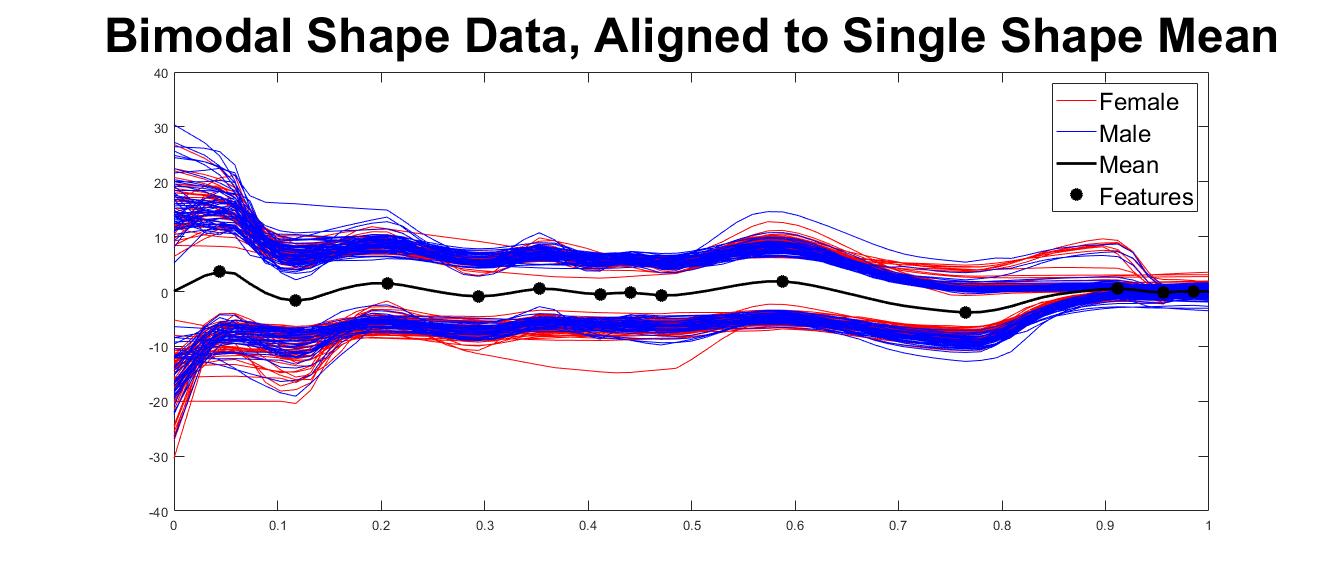
\includegraphics[width = .7\linewidth]{./Aligned_2_cluster.png}
	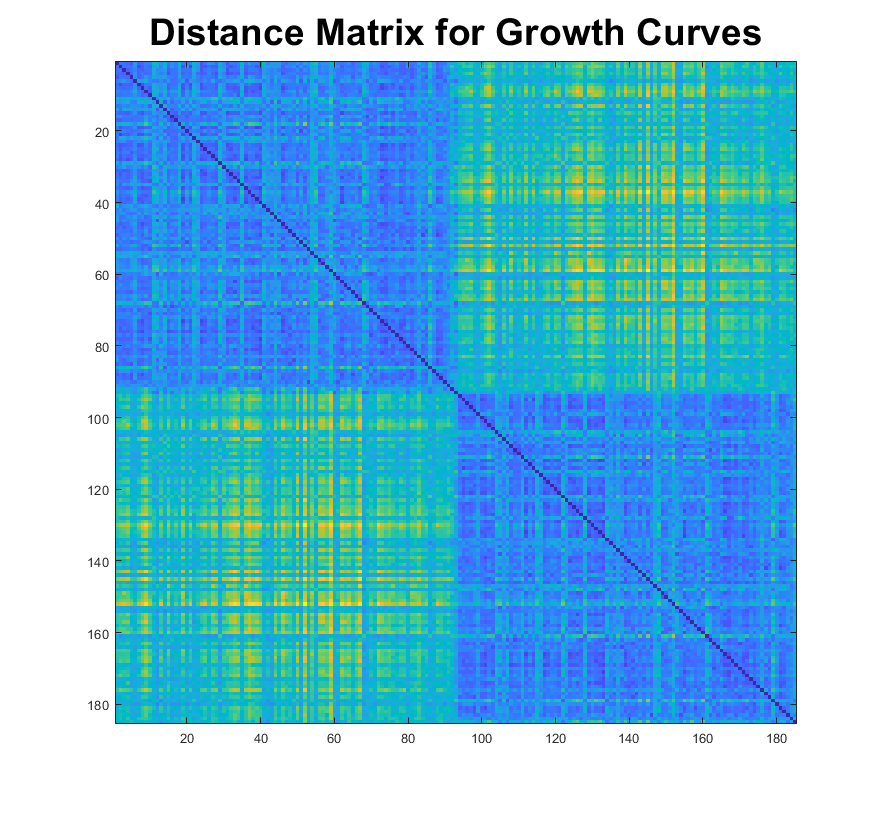
\includegraphics[width = .3\linewidth]{./Distance Matrix.png}
	\caption{This is the caption}
	\label{aligned function2}
\end{figure}

%\begin{figure}[h!]
%	\begin{center}	
	
%	\caption{This is the caption}
%	\label{distance matrix}		
%	\end{center}
%\end{figure}

\subsection{DTMRI Data}\label{DTMRI}

This analysis differs from our previous analysis in that we take a more general learning approach for both alignment and feature extraction. Because we don't have a multiple alignment approach for our DTMRI data, we instead treat each subject as a possible cluster 'median', align other subjects individually, and then learn which medians produce informative feature spaces. Secondly, in our previous examples, our feature extraction was non-parametric. In this case, rather than learning optimally informative features, we learn optimally informative feature representations, which for this example corresponds to within region clustering, (parameterized by k for k-means).



The basic pipeline is as follows;\\

\noindent
For each subject;\\
1) Domain Adaption: Pairwise Functional Optimal Transport with all other subjects\\
2) Feature Extraction: $k$-means\\
3) Feature Selection: Select optimal $k$ based on 1-cut Decision Tree test set accuracy\\
4) Classification: Decision Tree, $maxNumCuts = 4$\\


\end{document}



